\chapter{Ensemble Learning and Stacked Generalization} \label{chap:ensemble}

\section*{}

This chapter provides an overview over the concepts of Ensemble Learning and Stacked Generalization.

The field of \textit{Ensemble Learning} is presented briefly, with examples of general as well as more specific approaches used in the field of Anomaly Detection. 
Finally, the concept of \textit{Stacked Generalization} is presented as well as several approaches that are used in this field.

\section{Ensemble Learning Definition}\label{sec:ensemble_def}

Based on the definition provided by \textcite{Mendes-Moreira2012}, Ensemble Learning can be defined as:

\begin{definition}[Ensemble Learning] \label{def:ensemble_learning}
	Ensemble Learning is a process that uses a set of models (ensemble), each of them obtained by applying a learning algorithm to a given problem. This set of models is integrated in some way to obtain the final output.
\end{definition}

It is important to note that this definition is independent of the learning mode, which means that Ensemble Learning can be used for supervised and unsupervised learning \cite{Mendes-Moreira2012}.
Although Ensemble Learning is more frequently applied in supervised learning (classification and regression), it has also been used in clustering \cite{Strehl:2003:CEK:944919.944935}.

However, given the wide scope of these applications, this chapter and the following ones will only focus on classification applications of Ensemble Learning.

Formally, a classification model (or hypothesis) $m = (L, P, \mathcal{D})$ is an application of a learning algorithm $L$, with a set of defined parameters $P$ and trained on a dataset $\mathcal{D} = \{(x_i, y_i), i = 1, \dots, N\ \}$, where $x_n$ represents the feature values of the $n^{th}$ instance and $y_n$ the class value of the $n^{th}$ instance.
%\textbf{COMPLETAR} Each instance $x_i$ has $M$ features
Given a data instance $x_i$ from a dataset $\mathcal{D}$, $m(x_i)$ is the prediction of the class value of $x_i$ made by model $m$.

Therefore, an ensemble $E = \{m_j, j = 1, \dots, J \}$ can be defined as a set of $J$ models, where $E(x_i) = g(m_1, \dots, m_J)$ corresponds to the prediction of the class value of $x_i$ by the ensemble $E$. This prediction is made using an aggregation function $g$ which combines the predictions from the $J$ models of the ensemble, $m_1(x_i), m_2(x_i), \ldots, m_J(x_i)$.
It is important to mention that this definition is recursive, as an ensemble can also be considered a model in another ensemble.
The different ways in which the set of models can obtained and then integrated to obtain a final output will be discussed further in this section.

%It is important to mention that this definition is recursive, as an ensemble can also be considered a model in another ensemble.

It is also important to refer that approaches with \textit{Multiple Models} or \textit{Multiple Learners} presented sometimes throughout the literature refer to the same concept presented in this section \cite{Mendes-Moreira2012}.

\textcite{Dietterich1990} presents three reasons why Ensemble Learning can lead to better results:

\begin{itemize}
	\item Applying a learning algorithm to a specific problem can be interpreted as searching for the best model for this problem (the one that is considered the \textit{best} according to a predefined metric) within a space of possible models $\mathcal{H}$. When the dataset provided is too small compared to the space $\mathcal{H}$, several models can be equally considered the \textit{best}. By building an ensemble of this set of models, it is possible to obtain a new model that may generalize better to new data.
	
	\item Some learning algorithms generate models for a specific problem by performing an optimization process over an error function, which can get stuck at a local minimum. This is the case, for example, of neural network algorithms. By building an ensemble of different models (obtained by starting this optimization at a different starting points), it is possible to obtain a model that is closer to the global minimum.
	
	\item Given a specific problem, a learning algorithm works by instantiating a model the mimics the underlying process that can explain this problem (we will represent this process by $f$). However, some learning algorithms (e.g. linear algorithms) may not have a model space $\mathcal{H}$ large enough to contain a model that can represent $f$ accurately. By building an ensemble of different models and combining their outputs, it may be possible to expand the model space $\mathcal{H}$ and have a better approximation of $f$.
\end{itemize}

\textcite{hansen1990neural} however state that there are two necessary (and sufficient) conditions for an ensemble of models to be more accurate than any of individual models that belong to it:

\begin{itemize}
	\item Each of the models that compose the ensemble must be \textit{accurate}, which according to the author is to be better than random guessing.
	
	\item The ensemble of models should be \textit{diverse} (i.e. the outputs of the models should be uncorrelated to each other).
\end{itemize}

\section{Ensemble Learning Process}

\textcite{Mendes-Moreira2012} proposes three phases to be considered when using Ensemble Learning (illustrated in figure~\ref{fig:ensemble_process}), which will be detailed in this section. 

\begin{figure}[ht!]
	\centering
	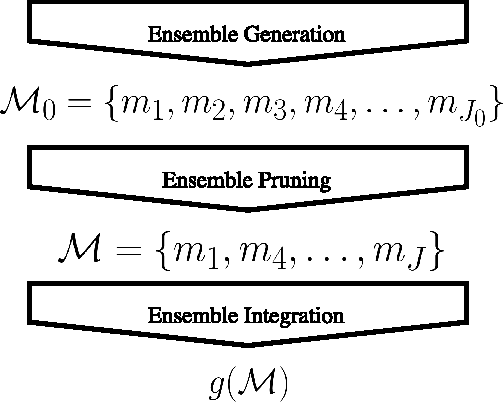
\includegraphics[width=0.5\textwidth]{figures/Ensemble_Process.pdf}
	\caption{Scheme representing the Ensemble Process. Adapted from \cite{Mendes-Moreira2012}.}
	\label{fig:ensemble_process}
\end{figure}

\subsection{Ensemble Generation}\label{sec:ens_gen}

The initial step in the process of Ensemble Learning is to generate an ensemble of models. We are interested in generating a set of models $\mathcal{M}_0 = \{ m_j, j = 1, \dots, J_0 \}$.

Ensembles can be of two different types \cite{Mendes-Moreira2012}:

\begin{itemize}
	\item \textit{Homogeneous}: when the set of models are generated by the same learning algorithm (e.g. tuned with different parameter settings). Most of the research work in Ensemble Learning is conducted with this type of ensembles \cite{Mendes-Moreira2012}.
	\item \textit{Heterogeneous}: when the set of models are generated by different learning algorithms. This type of ensembles may have more diversity between models than the homogeneous type, if the nature of the learning algorithms is diverse enough \cite{Mendes-Moreira2012}.
\end{itemize}

It is interesting to note that homogeneous ensembles can be used in heterogeneous ensembles, given the recursive definition of an ensemble.

A possible methodology that can be followed is the \textit{overproduce-and-choose} approach.
In this methodology a high number of models are generated in the ensemble generation phase (``overproduce''), leaving the task of selecting the best models to the pruning phase (``choose'').	

\textcite{Mendes-Moreira2012} presents different ways to produce different models in both homogeneous and heterogeneous ensembles, which will be detailed in this section.

\subsubsection{Data Manipulation Approaches}\label{sec:data_manipulation}

In the definition of a model $m = (L, P, \mathcal{D})$, these approaches perform changes in the dataset $\mathcal{D}$ used to train the learning algorithm $L$. The same learning algorithm is trained with different datasets will result in different models (which may or may not be diverse among themselves, depending on the sensitivity of the algorithm and its sensibility to the training dataset).

\paragraph{Subsampling from the Training Set}\mbox{}

This type of approach generates different models using different subsamples of the same dataset.
One of the most popular approaches is $bagging$ (bootstrap aggregating), which generates $k$ subsamples of a dataset $\mathcal{D}$.
These subsamples are made with replacement (a subsample can contain a data instance more than once).
A model is then trained with each of the $k$ subsamples generated, generating $k$ different models.

\paragraph{Manipulating the Input Features}\mbox{}

This type of approach can be divided in two subtypes:

\begin{itemize}
	\item \textit{Feature Selection}: 
	A feature selection process is performed on the dataset, in order to generate different datasets (each one with a different subset of features).
	One example of this approach is the \textit{random subspace} method \cite{ho1998random} (which chooses randomly feature subsets randomly).
	
	\item \textit{Feature Transformation}:
	A transformation is conducted on the features' original values, in order to generate different datasets with different features.
	One example is the \textit{input smearing} approach \cite{Frank2006} that adds gaussian \textit{noise} to each numeric feature.
\end{itemize}

\textit{Rotation forests} (proposed by \textcite{1677518}) incorporates both feature selection and transformation processes. First, this method selects different $k$ disjoint subsamples of features. Then, for every subsample, PCA is performed to project the feature space into a new one, where the new features correspond to linear combinations of the original ones.

\subsubsection{Model Generation Manipulation}

This type of approaches manipulates the learning algorithm's parameters or learning conditions.

\paragraph{Manipulating the Parameter Set}\mbox{}

Manipulating the parameter set of a learning algorithm is a possibility to generate different models, either by iterating by ranges of possible values (Grid Search \cite{hsu2003practical}) or using a Random Search \cite{bergstra2012random}.

\paragraph{Manipulating the Induction Process}\mbox{}

In order to to obtain a model $m$ from a learning algorithm $L$ on a dataset $\mathcal{D}$ it is necessary to perform \textit{induction}. This type of approaches try to change the way in which the model is generated, allowing the generation of models under different induction conditions.
One of the most common approaches is to change the error function in optimization-based learning algorithms (such as neural networks).

\paragraph{Manipulating the Generated Model}\mbox{}

This type of approaches performs adjustments on an already generated model, leading to different models.
One known approach is to change a Classification Association Rules (CARs) model by subsampling the model's set of rules $n$ times, generating $n$ models with different sets of rules. 

\subsection{Ensemble Pruning}

The generation of an ensemble in the previous phase, although might guarantee a wide diversity of models, it does not guarantee that the smallest ensemble possible with maximum accuracy was obtained. Several of the models may also have very correlated outputs, which do not add any extra knowledge to the final prediction.
Also, since some of the approaches for generating ensembles involve randomness, there is no guarantee all the models in the ensemble will contribute positively to the final prediction.

Therefore the goal of Ensemble Pruning is to improve the predictive accuracy of the ensemble and reduce the \textit{cost} of the ensemble (since an ensemble with a higher number of models will be more computationally costly to use).

Ensemble Pruning consists in selecting a subset $\mathcal{M}$ with $J$ models of the set of models generated in the previous step.
This phase corresponds to the ``choose'' step of the \textit{overproduce-and-choose} methodology presented in section \ref{sec:ens_gen}. Therefore:

\begin{equation}
\mathcal{M} \subseteq \mathcal{M}_0
\end{equation}

% DESCOMENTAR
%A possible heuristic to choose the models can be, for example, based on a combination of diversity and/or accuracy of the models. Several metrics suitable for measuring diversity and accuracy will be discussed further in this chapter, in section \textbf{PREENCHER COM A SECTION}.

\textcite{Mendes-Moreira2012} proposes two types of approaches for conducting Ensemble Pruning, which will be detailed in this section.

\subsubsection{Partition-Based Approaches}

The main idea of partition-based approaches is to cluster the models into several groups. This could be done, for example, with the clustering algorithm k-means, in order to obtain a set of clusters of similar models.
Afterwards, one or more representative models from each group are chosen to constitute the pruned ensemble.

\subsubsection{Search-Based Approaches}

Search-based approaches can divided in three different types:

\begin{itemize}
	\item \textit{Exponential Search Approaches}: Exponential Search Approaches search the complete search space of possible models to be included from $\mathcal{M}_0$. This search space has $2^{J_0} - 1$ possible subsets of models and the search for the optimal subset is an NP-complete problem.
	
	\item \textit{Randomized Search Approaches}: Randomized Search Approaches perform a heuristic search in the search space (e.g. using evolutionary algorithms). Approaches such as genetic algorithms, tabu search and population-based incremental learning have been used in previous works \cite{Ruta2001}.
	
	\item \textit{Sequential Search Approaches}: Sequential Search Approaches perform a search by iteratively adding and/or removing a model from subset to maximize some criteria.
	This can be done using using \textit{Forward Subset Selection}, \textit{Backward Subset Selection} or a combination of both.
	In \textit{Forward Subset Selection}, the search starts with am empty ensemble and models are iteratively added.
	In the case of \textit{Backward Subset Selection}, the search starts with all the possible models generated in the ensemble and they are iteratively removed.
\end{itemize}

\subsection{Ensemble Integration}\label{sec:ensemble_integration}

The final step in Ensemble Learning is the combination of the predictions from the models in the ensemble.

In classification, the most popular approaches to combine models can be divided into two categories: combination-based approaches and model-based approaches.

\subsubsection{Combination-based Approaches}

Combination-based approaches are based on combination rules of the class values outputted by the models in the ensemble.
First it is important to define the decision of the $j^{th}$ model (referred in section \ref{sec:ensemble_def} as \textit{class value}) as $d_{j,c} \in \{ 0,1 \}, j = 1, \dots, J$ and $c = 1, \dots, C$, where $J$ is the number of models in the ensemble (as defined previously in section \ref{sec:ensemble_def}) and $C$ is the number of classes.
If the $j^{th}$ model outputs class $c$, then $d_{j,c} = 1$ and 0 otherwise.

\paragraph{Majority Voting}\mbox{}

Majority Voting has three different subtypes, in which the ensemble output corresponds to the class predicted by all classifiers (\textit{unanimous voting}), the class predicted by at least one more than half the number of classifiers (\textit{simple majority}) or the class predicted by the majority  of the classifiers, even if it is predicted by less than half of the number of classifiers (\textit{plurality voting}) \cite{Polikar2012a}.

The Majority Voting approach (unless specified otherwise) usual refers to \textit{plurality voting} \cite{Polikar2012a} and the decision of which class value to output can be defined as follows: 

\begin{equation}\label{eq:majority}
\text{arg}\max_c \sum_{j = 1}^{J} d_{j,c}
\end{equation}

\paragraph{Weighted Majority Voting}\mbox{}

If it is known that some of the models are more likely to make correct predictions than others, weighting the decisions of the models can improve the performance of the Majority Voting approach \cite{Polikar2012a}.
In this case, models with higher performance would have a bigger weight assigned and models with a worse performance otherwise.
We define the weight of a model $m_j$ as $w_j$.
These weights usually are normalized so that:

\begin{equation}
w_j \in [0, 1] \ \wedge \ \sum_{c = 1}^{C} w_{j} = 1, \ j = 1, \dots, J
\end{equation}

In this case, the decision of the class output is defined as follows:

\begin{equation}
\text{arg}\max_c \sum_{j = 1}^{J} w_j \cdot d_{j,c}
\end{equation}

A estimation of the weights could be performed by estimating the models' generalization performance in a separate validation set.

\paragraph{Borda Count}\mbox{}

The Board Count method assumes that each model is capable of ranking its support to each class $c$ and takes this into consideration \cite{Polikar2012a}. This method can be particularly useful in multi-class problems where $C$ takes a considerable value.

For each model $m_j$, each class $c$ receives $C-r$ votes being $r$ the position of $c$ in the ranking belonging to model $m_i$.
For example, if $C = 4$ and the class 1 is ranked $3^{rd}$ by model $m_1$ (meaning that model $m_1$ picked class 1 as being the third most probable), then class 1 will receive $4-3 = 1$ votes.
This procedure is then executed for each model and possible class value, the results are added up and the class with higher number of votes is chosen.

\subsubsection{Model-based Approaches}

Throughout the literature in Ensemble Learning, several more complex methods of prediction combinations are described \cite{Polikar2012a}.
Some of these can be considered model-based, in the sense that there is a training phase of an algorithm that ``learns'' how to combine the several models in the ensemble.
We will describe briefly two possible approaches in this section.

\paragraph{Stacked Generalization}\mbox{}

\begin{figure}[ht!]
	\centering
	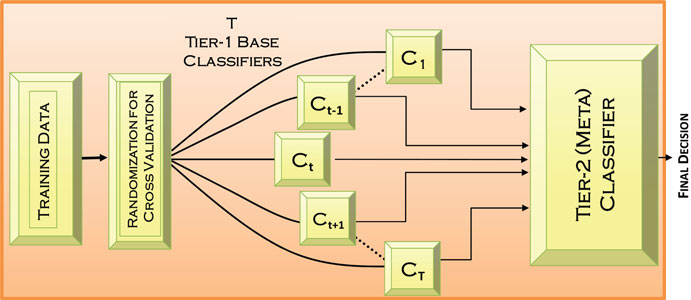
\includegraphics[width=0.8\textwidth]{figures/stacking}
	\caption{Scheme of the Stacked Generalization approach. Source: \cite{Polikar2012a}.}
	\label{fig:stacking}
\end{figure}

Stacked Generalization (also known as Stacking) is an Ensemble Learning method in which the predictions of the models are combined using another model (also known as a \textit{meta-classifier}) \cite{Polikar2012a}. In order to do so, a new dataset is generated using the prediction outputs of the models belonging to the ensemble.
This new dataset is then used to generate another model (the \textit{meta-classifier}).
This mechanism is illustrated in figure \ref{fig:stacking}.

This approach can be seen as an extension of the Weighted Majority Voting.
However, unlike this method, the impact of each model in the final decision is not translated into a single value.
Stacking determines which models are likely to be accurate in different parts of a dataset's feature space, since certain models may be more ``specialized'' in predicting correctly certain data instances.
In this case the predictions of these models for these data instances will have a higher ``weight'' and the remaining models a lower one.

Since this approach is the main focus of this dissertation, we will focus on it later in this chapter.

\paragraph{Mixture of Experts}\mbox{}

\begin{figure}[ht!]
	\centering
	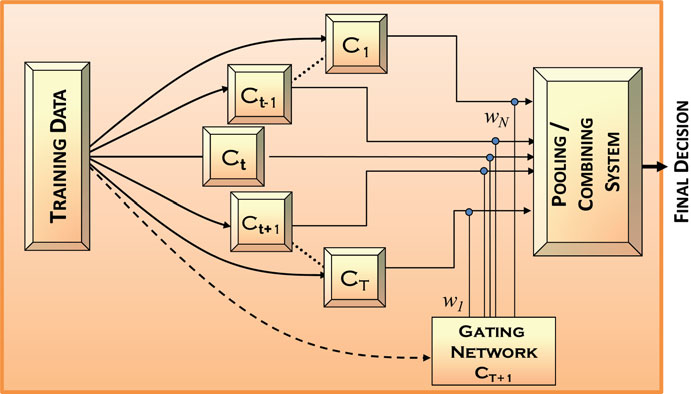
\includegraphics[width=0.8\textwidth]{figures/mixture_models}
	\caption{Scheme of the Mixture of Experts approach. Source: \cite{Polikar2012a}.}
	\label{fig:mixture}
\end{figure}

As the name reflects, the Mixture of Experts approach assumes certain individual models may be \textit{experts} in predicting the class value for certain data instances but more inaccurate for the remaining ones in the dataset. This background idea is very similar to the one behind Stacking, in which weights are assigned to each model of the ensemble reflecting its accuracy in certain parts of the dataset's feature set.

However, these weights are not determined by a new model but by a \textit{gating network} (as illustrated in \ref{fig:mixture}).
This gating network is trained using the expectation-maximization (EM) algorithm on the original dataset.

\section{Ensemble Learning Applications to Anomaly Detection}

Ensemble Learning has been previously used with Anomaly Detection techniques \cite{Aggarwal:2013:OA:2436823}.
Because these applications were typically based on unsupervised learning, we will focus on these in this section.
Several applications using Stacking (and therefore supervised learning based) will be discussed in the next section.
%We distinguish two types of approaches, based on the learning mode of the Anomaly Detection techniques: supervised learning approaches and unsupervised learning approaches.


%\subsection{Supervised Learning Approaches}

\subsection{Unsupervised Learning Approaches}

%The majority of applications of Ensemble Learning to Anomaly Detection are associated with unsupervised learning approaches.
\textcite{Aggarwal:2013:OA:2436823} classifies unsupervised learning approaches as being either sequential or independent.

\subsubsection{Sequential Approaches}

In sequential approaches, several models are applied sequentially either to the entire dataset or portions of it \cite{Aggarwal:2013:OA:2436823}.
The underlying assumption of this group of approaches is that the application of each algorithm allows a more refined execution by either modifying the data or the subsequent models.
Data modifications could include some of the approaches described in section~\ref{sec:data_manipulation}, such as subsampling the dataset, performing feature selection and feature transformation \cite{Aggarwal:2013:OA:2436823}.
The final decision can be either the decision of the last applied model or a combination of the several models applied.

Models in earlier stages of a sequential approach could, for example, remove more obvious \textit{anomalous} instances of the data so that latter models perform a more robust anomaly detection {\cite{Aggarwal:2013:OA:2436823}.
The latter might then be able to have a better understanding of less-noticeable \textit{anomalous} instances the data.
This can be used, for example, with clustering based techniques, in which more robust clusters can be built after the most \textit{anomalous} instances are removed \cite{Barbara:2003:BDM:952532.952616}.

\subsubsection{Independent Approaches}

In independent approaches, several models are used without having any effect on one another.
These models can be applied either to the entire dataset or to portions of it \cite{Aggarwal:2013:OA:2436823}.
The underlying assumption of these approaches is that several Anomaly Detection techniques can be specialized on certain instances of the dataset, so therefore an application of these techniques and consequent combination of predictions might lead to more accurate decision.
The methodologies to generate the models in these approaches include some of the ones already described in section~\ref{sec:ens_gen}, such as feature selection and dataset subsampling.

Some approaches within this category use models with the LOF (\cite{Breunig:2000:LID:335191.335388}) and LOCI (\cite{PapadimitriouS.KitagawaH.2003}) learning algorithms.	

\subsubsection{Ensemble Integration}

One of the difficulties with unsupervised learning Anomaly Detection techniques is that they usually output a numeric score.
Different techniques can output scores in different scales as, some techniques might output a normalized score (e.g. LOF), where others might output a raw distance score (e.g. k-nearest neighbor) \cite{Aggarwal:2013:OA:2436823}.
Different techniques might also have a different ordering of the scores, as some techniques output larger scores for \textit{anomalous} instances, while others output smaller scores for this type of instances \cite{Aggarwal:2013:OA:2436823}.
Therefore, it is important to normalize the scores of each technique so that they can be meaningfully combined without over-weighting specific techniques \cite{Aggarwal:2013:OA:2436823}.

\paragraph{Normalization of Scores}\mbox{}

The first step is to make sure that each model of the ensemble has the same ordering of the scores.
This can be solved by flipping the sign of the scores of the models in which lower score values correspond to higher probability of being an anomalous data instance.
By doing this, in every technique a higher score will always correspond to a higher probability of a data instance being anomalous.

The second step is to convert the scores of the different models into comparable values.
\textcite{Aggarwal:2013:OA:2436823} presents two possible methods:

\begin{itemize}
	\item \textit{Range-based scaling}:
	Range-based scale uses the maximum and minimum scores of one model for a specific dataset to convert the scores.
	The converted scores will then lie in the interval $[0,1]$.
	
	Let $s_j(x_i)$ the score that the model $m_j$ outputs for a data instance $x_i$ and let $max_{j}$ and $min_{j}$ be the maximum and minimum value respectively of the scores of model $m_j$ for a dataset $\mathcal{D}$.
	The converted score of a data instance $x_i$ with a model $m_j$ takes the following value $s'(x_i)$: 
	
	\begin{equation}
	s_j'(x_i) = \frac{s_j(x_i) - min_j}
	{max_j - min_j}
	\end{equation}
	
	The disadvantage of this method is that the values of the converted scores will depend highly on the values of $max_j$ and $min_j$.
	For example, in most Anomaly Detection techniques the value of $max_j$ is attributed to the most \textit{anomalous} data instance.
	In some datasets this score might be much larger than the scores of the other data instances.
	This phenomena can reduce drastically the discrimination of the remaining scores and reduce the ability of distinguishing which ones might be \textit{anomalous} \cite{Aggarwal:2013:OA:2436823}.
	
	\item \textit{Standardization}: 
	Standardization converts the scores into standard scores (also known as Z-values).
	
	Let $\mu_j$ and $\sigma_j$ be the mean value and standard deviation respectively of the scores of model $m_j$ for a dataset $\mathcal{D}$.	
	The converted score of a data instance $x_i$ with a model $m_j$ takes the following value $s_j'(x_i)$:
	
	\begin{equation}\label{eq:standardization}
	s_j'(x_i) = \frac{s_j(x_i) - \mu_j}{\sigma_j}
	\end{equation}
	
	This method however, assumes that the scores of each model $m_i$ follow a gaussian distribution. Although this assumption rarely holds, it is reported that this method usually provides reasonably robust results \cite{Aggarwal:2013:OA:2436823}.
	
\end{itemize}

Another method, discussed by \textcite{Gao:2006:COS:1193207.1193286}, is to convert the techniques' scores into probabilities using the EM algorithm.

\paragraph{Combination of Scores}\mbox{}

After the scores of the different techniques are normalized they can be combined.
Note that the approaches discussed in section~\ref{sec:ensemble_integration} can not be used, since the score is a real number and not a nominal number.

\textcite{Aggarwal:2013:OA:2436823} presents two possible combination methods:

\begin{itemize}
	\item \textit{Averaging}:
	The final score is computed as the mean of the scores of the different models. Therefore, a data instance $x_i$ will have the following score:
	
	\begin{equation}
	\frac{\sum_{j = 1}^J s_j(x_i)}{J} 
	\end{equation}
	
	\item \textit{Maximum}:
	The final score is computed as the maximum score across the different models. Therefore, a data instance $x_i$ will have the following score:
	
	\begin{equation}
	\max_{j} \ s_j(x_i) \ , \ j = 1, \dots, J 
	\end{equation}
	
\end{itemize}

\section{Stacked Generalization}\label{sec:stacking}

Stacked Generalization (also known as Stacking) was proposed initially by \textcite{wolpert1992stacked}.
It consists of an ensemble method with three steps: 1) models are generated using one or more learning processes; 2) a new dataset is generated with the predictions of those models, together with the original target variable; and 3) a new model is obtained using the new dataset containing the predictions of the previous models~\cite{Sesmero2015}.
We refer to the models in the ensemble as the \textit{level-0 models}, their outputs as \textit{metafeatures} and the model built with them as the \textit{level-1 model} or \textit{meta-classifier}.

%\textbf{MUDAR J e F PARA OUTRA LETRA}
Formally, given a dataset $\mathcal{D}^0$, Stacking first generates a set of mutually exclusive partitions of approximate size $\mathcal{D}^0_1, \dots, \mathcal{D}^0_Z$. Then, similarly to a \textit{Z}-fold cross-validation procedure, at each iteration $z$, the method omits the subset $D^0_z$ and uses the subset $D^0 - D^0_z$ as a training set to generate $M$ level-0 models by training several learning algorithms.%
After the level-0 models have been generated for each
iteration $z$, they are applied to the dataset $D_z$ to obtain the predictions that will be used as the level-1 dataset values. We will refer to this dataset as the meta-dataset $\mathcal{D}^1_z$. The process is repeated for all $Z$ datasets and the complete level-1 dataset, $D^1$ is defined as:

\begin{equation}
\bigcup\limits_{z=1}^{Z} \mathcal{D}^0_z
\end{equation}

The dataset $\mathcal{D}^1$ has the same number of rows as $\mathcal{D}^0$, but $M$ features (whose values are the predictions of the $M$ level-0 models) plus the class value.
The dataset $\mathcal{D}^1$ can then be used to train a learning algorithm, which becomes the level-1 model~\cite{Sesmero2015}.

To classify a new instance $x_i$, the level-0 models produce a vector of predictions ${m_1(x_i), \dots, m_M(x_i)}$.
This vector is the input to the level-1 model, which makes a prediction regarding the class value of $x_i$.

\subsection{Applications to Anomaly Detection}

The application of Stacking for Anomaly Detection is recent and sometimes not very transparent and easy to track.
However, we can emphasize two approaches in the literature:

\begin{itemize}
	\item \textcite{Micenkova} presented a Stacking Generalization methodology for Anomaly Detection, using outputs from two unsupervised Anomaly Detection techniques (k-NN outlier and LOF).
	Among with these two techniques, the authors used feature bagging which consists in a feature selection approach to generate different models from the same learning algorithms.
	The meta-classifier used in this approach was a model based on the Logistic Regression learning algorithm with L1 Regularization.
	
	\item \textcite{Cerqueira2016} proposed an approach similar to Stacking, in which the predictions from several models (LOF and Hierarchical Agglomerative Clustering) were added to the original dataset. According to our notation, the dataset used in this work has the features from $\mathcal{D}^0$ and $\mathcal{D}^1$.
	The meta-classifier used in this approach was a model based on the XGBoost learning algorithm.
\end{itemize}

%lala
